\documentclass[a4paper,11pt]{article}
\usepackage[utf8]{inputenc}
\usepackage[english]{babel}
\usepackage{float}
\usepackage{amsfonts}
\usepackage{amsmath,array}
\usepackage{booktabs}
\usepackage{amssymb}
\usepackage{nomencl}
\usepackage{graphicx}
\usepackage{multicol}

%% Proper
\usepackage{natbib}
\setcitestyle{round,authoryear}  
%%\bibliographystyle{plainnat}




\begin{document}
\title{Non-Stationary frequency adaptation of biases precipitation series}
\author{Cantalejo, M}
\maketitle
%%\tableofcontents
\abstract{URL: https://github.com/mcantalejoi/PROYECTO$\_$FINAL.git

The variability of forcings and associated hydrological processes, make Mediterranean basins of special interest as observatories of climate change.

The high seasonal variability cannot be adequately reproduced using the well-known 
empirical quantile mapping method. 

}


%\keywords{Keywords: Bias-adjustment,Uncertainty, rainfall-events, climate change}

\section{Introduction}\label{sec1}
Climate projections from the Coordinated Regional Downscaling Experiment over Europe present interesting estimations of climate change on a high spatial resolution  \cite{bib1}. Those available climate projections  from global circulation models (GCM), even regionalized, present important spatial and temporal limitations zones such as the Mediterranean, which have significant impacts on flow regime \cite{bib2} , \cite{bib3}.

Different bias-correction techniques has been developed to reduce biases from climate projections. Within the different statistical techniques, Quantile mapping outstand reducing biases which are widely-used in hydrological impacts studies \cite{bib4}. It consisit in mapping each quantile of the empirical probability distribution (ECDF) from simulated historical series into each ECDF's quantile of the observations. The same correction is them applied to future climate projections \cite{bib5}. The application of this technique, is however, applied under the assumption of the stationary behavior. However, climatic variables such as precipitation, present an clear non-stationary patterns,in occurrence and amount of rainfall event, through the annual cycle \cite{bib6}. This works aims to study the impact of bias-correctiing precipitation occurrence by the application of Quantile Mapping. 

The paper is organized as follows. In section 3 the methodology and data avaiable is described. In sections 4 shows the results obtained from the application of the non-stationary method and a brief conclussion.  


\section{Data and methods}\label{sec2}
\subsection{Data} 
Daily precipitation measurements were obtained from meteorological station (no. 176) located near the coast of Salobreña (Granada, South Spain). The mean annual rainfall recorded for the period 1970 -2005 is 603 mm, with minimum and maximum values of 380 mm and 986 mm respectively. Precipitation data show a strong inter-annual variability through the year with rainfall events that reached 50 mm/day on winter to 5 mm/day on summer, as well as precipitation occurrence which is 10 times more frequent in winter than summer.

This available information was used in combination with a set of climate projections (GCM-RCMs) of the international coordinated framework for European regions (EURO-CORDEX).As the RCMs inherits the biases from the GCMs output, it is important to combine different global and regional scale models to obtain a reliable data base to assess uncertainty.  


\subsection{Methods} 
The methodology presented in this work can be subdivided into the following main steps: (i) the non-stationary analisys of rainfall frequency from modelled and observed precipitation (ii)the application of the non-stationary Frequency adaptation(ns-FA) and (iii) the validation of the unbiases series with observations.

\subsubsection{Non-Stationary analysis of rainfall frequency} 
The analysis of the rainfall frequency started with the definition of a wet-day threshold according to observations. This varies throughout the literature, from $p_{0}$> 0.1mm/day \cite{bib7} to $p_{0}$> 1mm/day \cite{bib8}. 

The adaptation of rainfall occurrence from simulations is successfully achieved by editing this threshold as a time-dependent parameter $p_{0}^{BC}$ (t)  , to ensure the same proportion of rainfall days throughout the year in both, observations and hindcast data series (1970-2000). 


\begin{figure}[H]  % H quiere decir aqui 'here' 
\centering
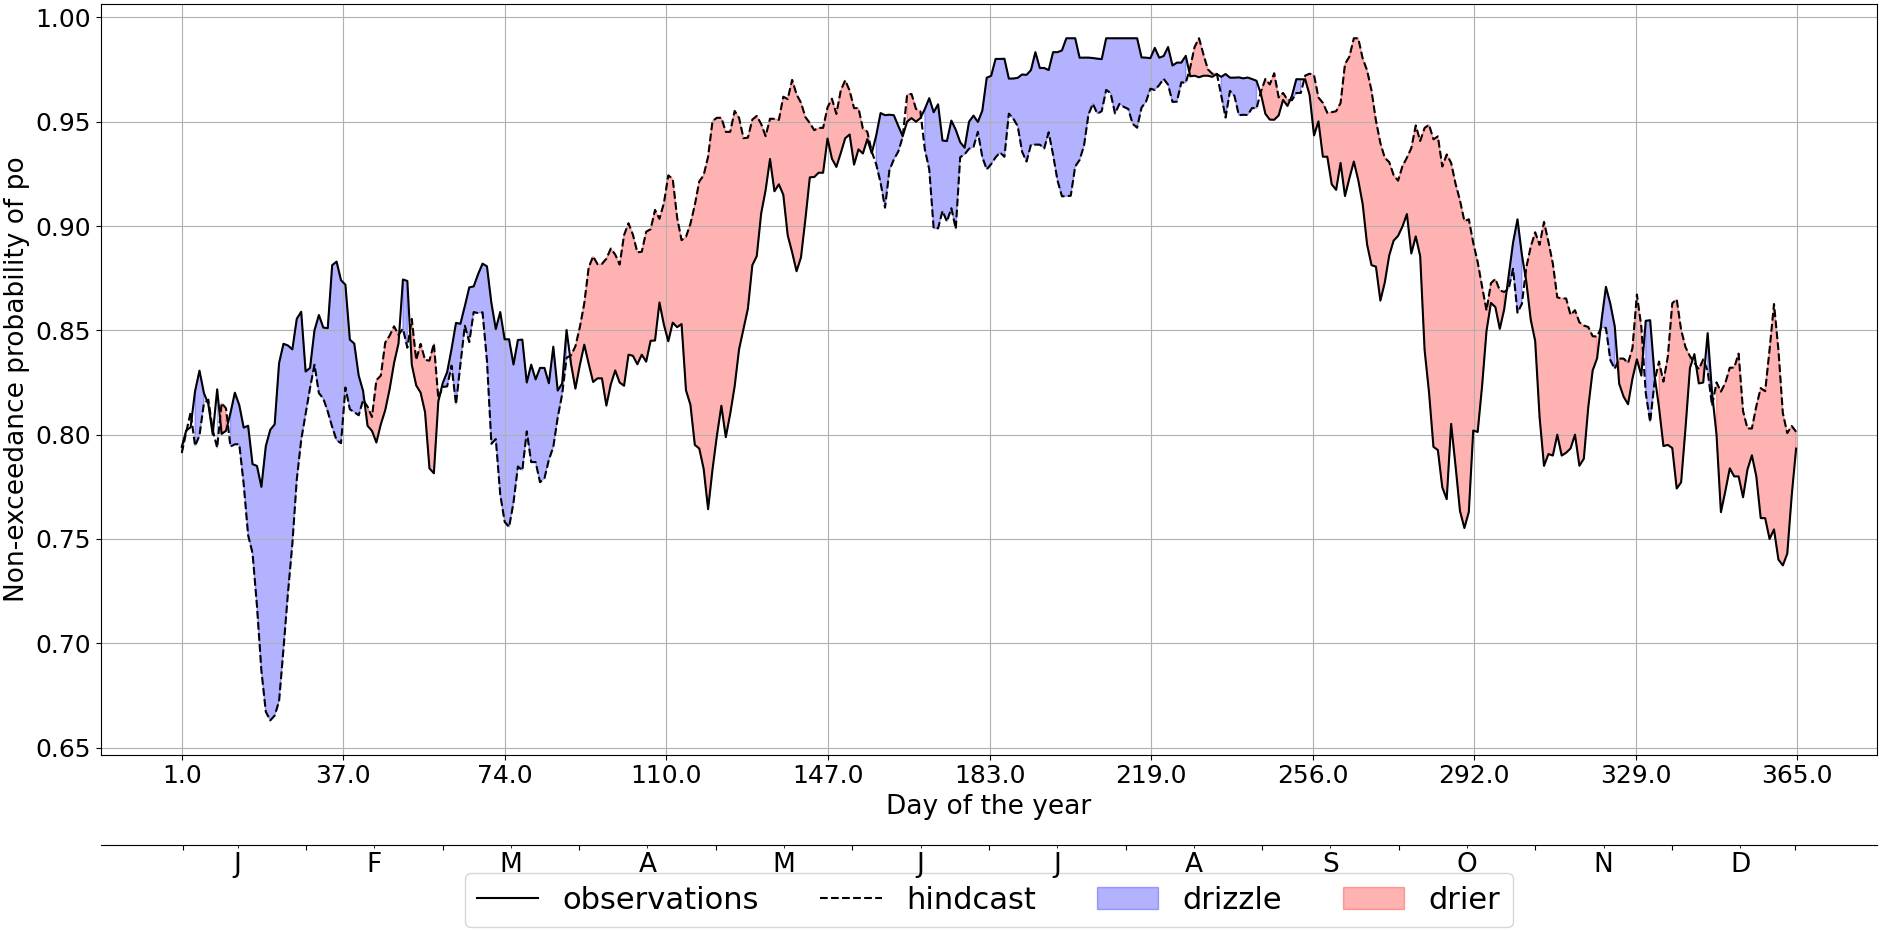
\includegraphics[scale=0.26]{Fig1.PNG}
\caption{. Iso-value curves of the non-exceedance probability precipitation of $p_{o}=$ 0.1 mm/day. Black solid line stands for observations, black dashed line stands for hindcast from SMHI-IPSL-IPSL-CM5A-MR. X-axis represents julian days and months. }
\label{F1}
\end{figure}


\subsubsection{Non-Stationary frequency adaptation} 
The adaptation of rainfall frequency to consider its non-stationary behavior has been reached from the following steps: (i) it is defined a constant threshold ($p_{0}$) of 0.1 mm/day to classify rainfall days ($p_{0}(t) < p(t)$) and dry days ($p(t) < p_{0}(t)$) in correspondence with the minimum recorded rainfall amount; (ii) it is obtained the ECDF, for each day of the year (t), for hindcast data $F(p_{0}  ,t)$ and observed data $F_{*} (p_{0}  ,t)$ for the set threshold ($p_{0}$), using a moving window of 7-days length.. Knowing $F_{*}(p_{0},t)$,  for a given t, it is obtained the time-dependent threshold ($p_0^{BC}(t)$) that it is necessary to apply to the hindcast/projections data to keep the same proportion of dry-wet days along the year than in observations following \ref{E1}.

\begin{equation}
p_0^{BC}(t) = F^{-1}(F_*(p_0,t),t)
\label{E1}
\end{equation}

\subsubsection{Quantifying performance} 
After applying \ref{E1} to remove non-stationary biases from hindcast and projected series, several diagnostic parameters proposed in the VALUE initiative, are used to validate the performance of the downscaling method: number of wet-days per month $n_{wet}$

To evaluate them, we employ the relative bias $\Delta$ \cite{bib9}, defined as $\Delta(m) =(\xi-\omega)/\omega \cdot 100$, where m refers to each month of the year, $\xi$ is the mean performance of each metric per month related to the simulated series during the reference period (1970-2000) and $\omega$ analogously for the observations. Simulated series could be referred to (a) raw simulations, (b)non-stationary corrected series, which allows to compare the biases-removal from each source of information. 

Due the variability between simulated series from the 9 GCM-RCMs selected, it is calculated the time-dependent error ($\delta$) for each station, reformulated as $ \lvert{\xi} - {\omega}\rvert \cdot 100/ \omega$, where ${\xi}$ is the average value of $\xi$ (referred to each RCM). The expression $\Delta(m)$ is then averaged between stations. For each season, is considered a three-month period were the mean ($\mu$) and the 95-level confidence interval (95CI) of the  $\Delta(m)$, were calculated as: 

\begin{equation}
\mu \pm t_{\alpha/2} \cdot \dfrac{\sigma}{\sqrt{n}}
\label{E2}
\end{equation}

where $\alpha$  refers to the level of the confidence interval (eg: $\alpha = 1 - 0.95 = 0.05$), and $\mu$ and $\sigma$ are respectively the mean and the standard deviation of the sample. The number of values for each sample (n=9), implies the use of a t-student distribution ($t_\alpha⁄2$) for the estimate of the 95CI. Analogue to $\Delta$, it is assessed the uncertainty of the projected changes ($\delta$), by associated mean ($\mu$) and the 95-level confidence interval (95CI). 


\section{Results}\label{sec4}

The $\mu$ from $\Delta n_{wet}$  and 95CI  is reduced from raw rainfall series to frequency adapted series by both approaches. The reduction achieved by the ns-FA is significant for all seasons, although the less reduction appears during summer. Another important aspect is the reduction obtained for the 95\% confident interval which means a higher agreement between corrected simulated series among different RCMs. In this sense, ns-FA also obtained a higher reduction of the uncertainty reaching the highest value on summer. 

\begin{table}[H]
%\begin{left}
\begin{minipage}{300pt}
\caption{Caption text}\label{tab1}%
\begin{tabular}{ccccc}

\toprule
Time-series & Dec-Feb & Mar-May & Jun-Aug & Sep-Nov \\
\midrule
raw RCM's    & 53\% (24\%) & 56\% (43\%)& 316\% (243\%)& 71\% (65\%) \\
ns-FA        & 4.7\% (2\%) & 5.8\% (2\%)& 17.7\% (6\%)& 6.4\% (2\%) \\

\end{tabular}
\end{minipage}
%\end{left}
\end{table}



\section{Bibliography}\label{sec5}

\bibliography{BIB}
\bibliographystyle{plainnat}
\nocite{*}
	
\end{document}

